\subsection{流动法(温差法)}
流动法生长晶体装置一般由三部分组成(图3.21):生长槽(育晶器)C,溶解槽A和过热槽B。三槽之间的温度是B槽的温度高于A槽的温度高于A槽的,而A槽的温度又高于C槽的,A槽中过剩的原料在不断地搅拌下溶解,使溶液在高于C槽的温度在饱和,然后经过滤器进入过热槽B。过热槽的温度一般高于生长槽温度5--10℃。可以充分溶解从溶解槽流入的微晶,以提高溶液的稳定性。经过过热后的溶液用泵打入生长槽C,C槽的溶液是过饱和的,保证晶体生长有一定的驱动力。由于晶体的生长,从而使变稀的溶液流到溶解槽溶解原料,使溶液重新达到饱和,溶液如此循环流动,晶体不断生长。晶体的生长速度受到溶液的流动速度和A,C两槽温差的控制。这种方法的优点是生长温度和过饱和度都固定。使晶体始终在最有利的温度和最合适的过饱和度下生长,避免了因生长温度和过饱和度变化而产生的杂质分凝不均匀和生长带等缺陷,使晶体完整性更好。流动发的另一个优点就是生长大批量的晶体和培养大单净不收溶解度和溶液体积的影响,只受生长容器大小的限制。日本大阪大学用这种方法长出400$\times$400$\times$600mm大KDP晶体,生长速度达2mm/d。流动法的缺点是设备比较复杂,调节三槽之间适当的温度梯度和溶液流速之间的关系需要有一定的经验。
\begin{figure}[h]
 \centering
 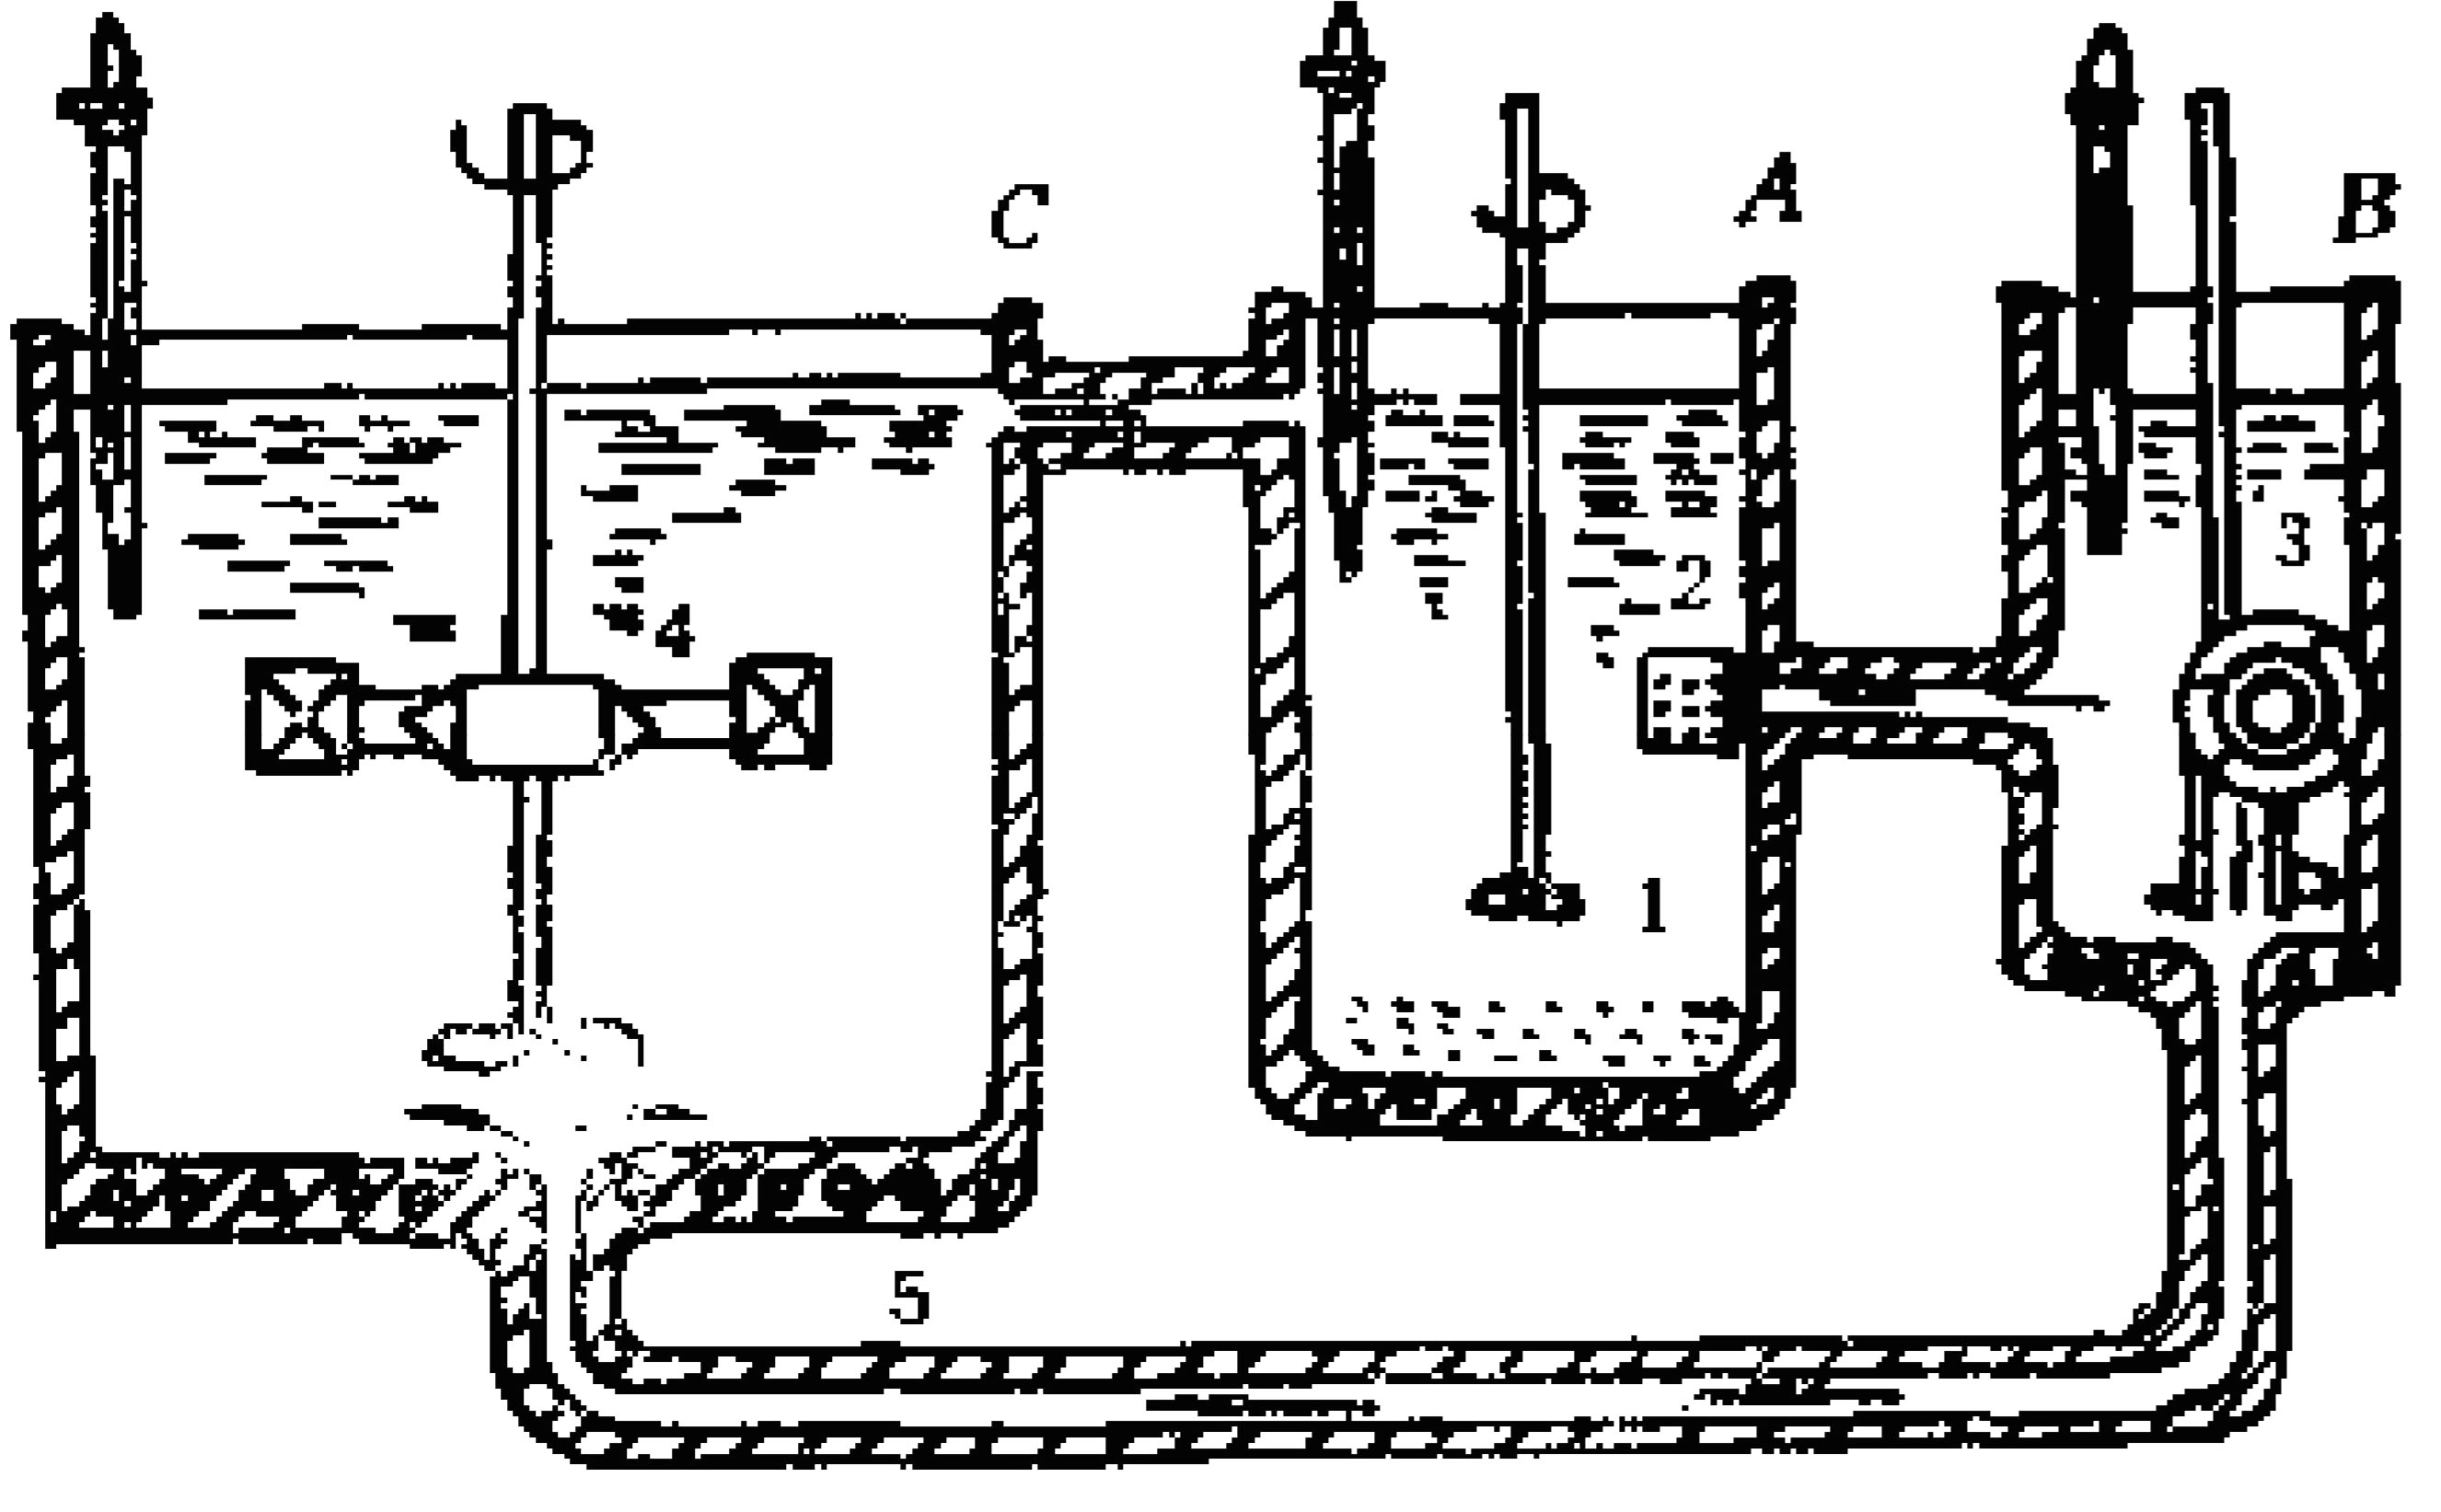
\includegraphics[width=0.6\textwidth]{fig/cp03/img3.21.jpg}
 \caption{循环流动育晶装置}
\end{figure}

采用适当装置也可以利用浓差自然对流来生长晶体。图3.22示出利用亚稳相和稳定相溶解度的差别通过浓差对流来生长$\alpha$-LiIO$_3$体的装置。两连通的玻璃槽,右边装$\beta$-LiIO$_3$原料,左边为生长槽,由于在20--30℃时,$\beta$-LiIO$_3$的溶解度比$\alpha$-LiIO$_3$的大1--2\%。浓度较大的LiIO$_3$溶液靠自然对流进入左边生长区,生长槽下部设置加热器,将溶液温度保持在40℃,造成对$\alpha$-LiIO$_3$的过饱和,析出的溶质在$\alpha$-LiIO$_3$种子上生长,变稀的溶液上升流回右边的原料槽重新溶解$\beta$-LiIO$_3$,原料槽靠空气冷却稳定在20--30℃。
\begin{figure}[h]
 \centering
 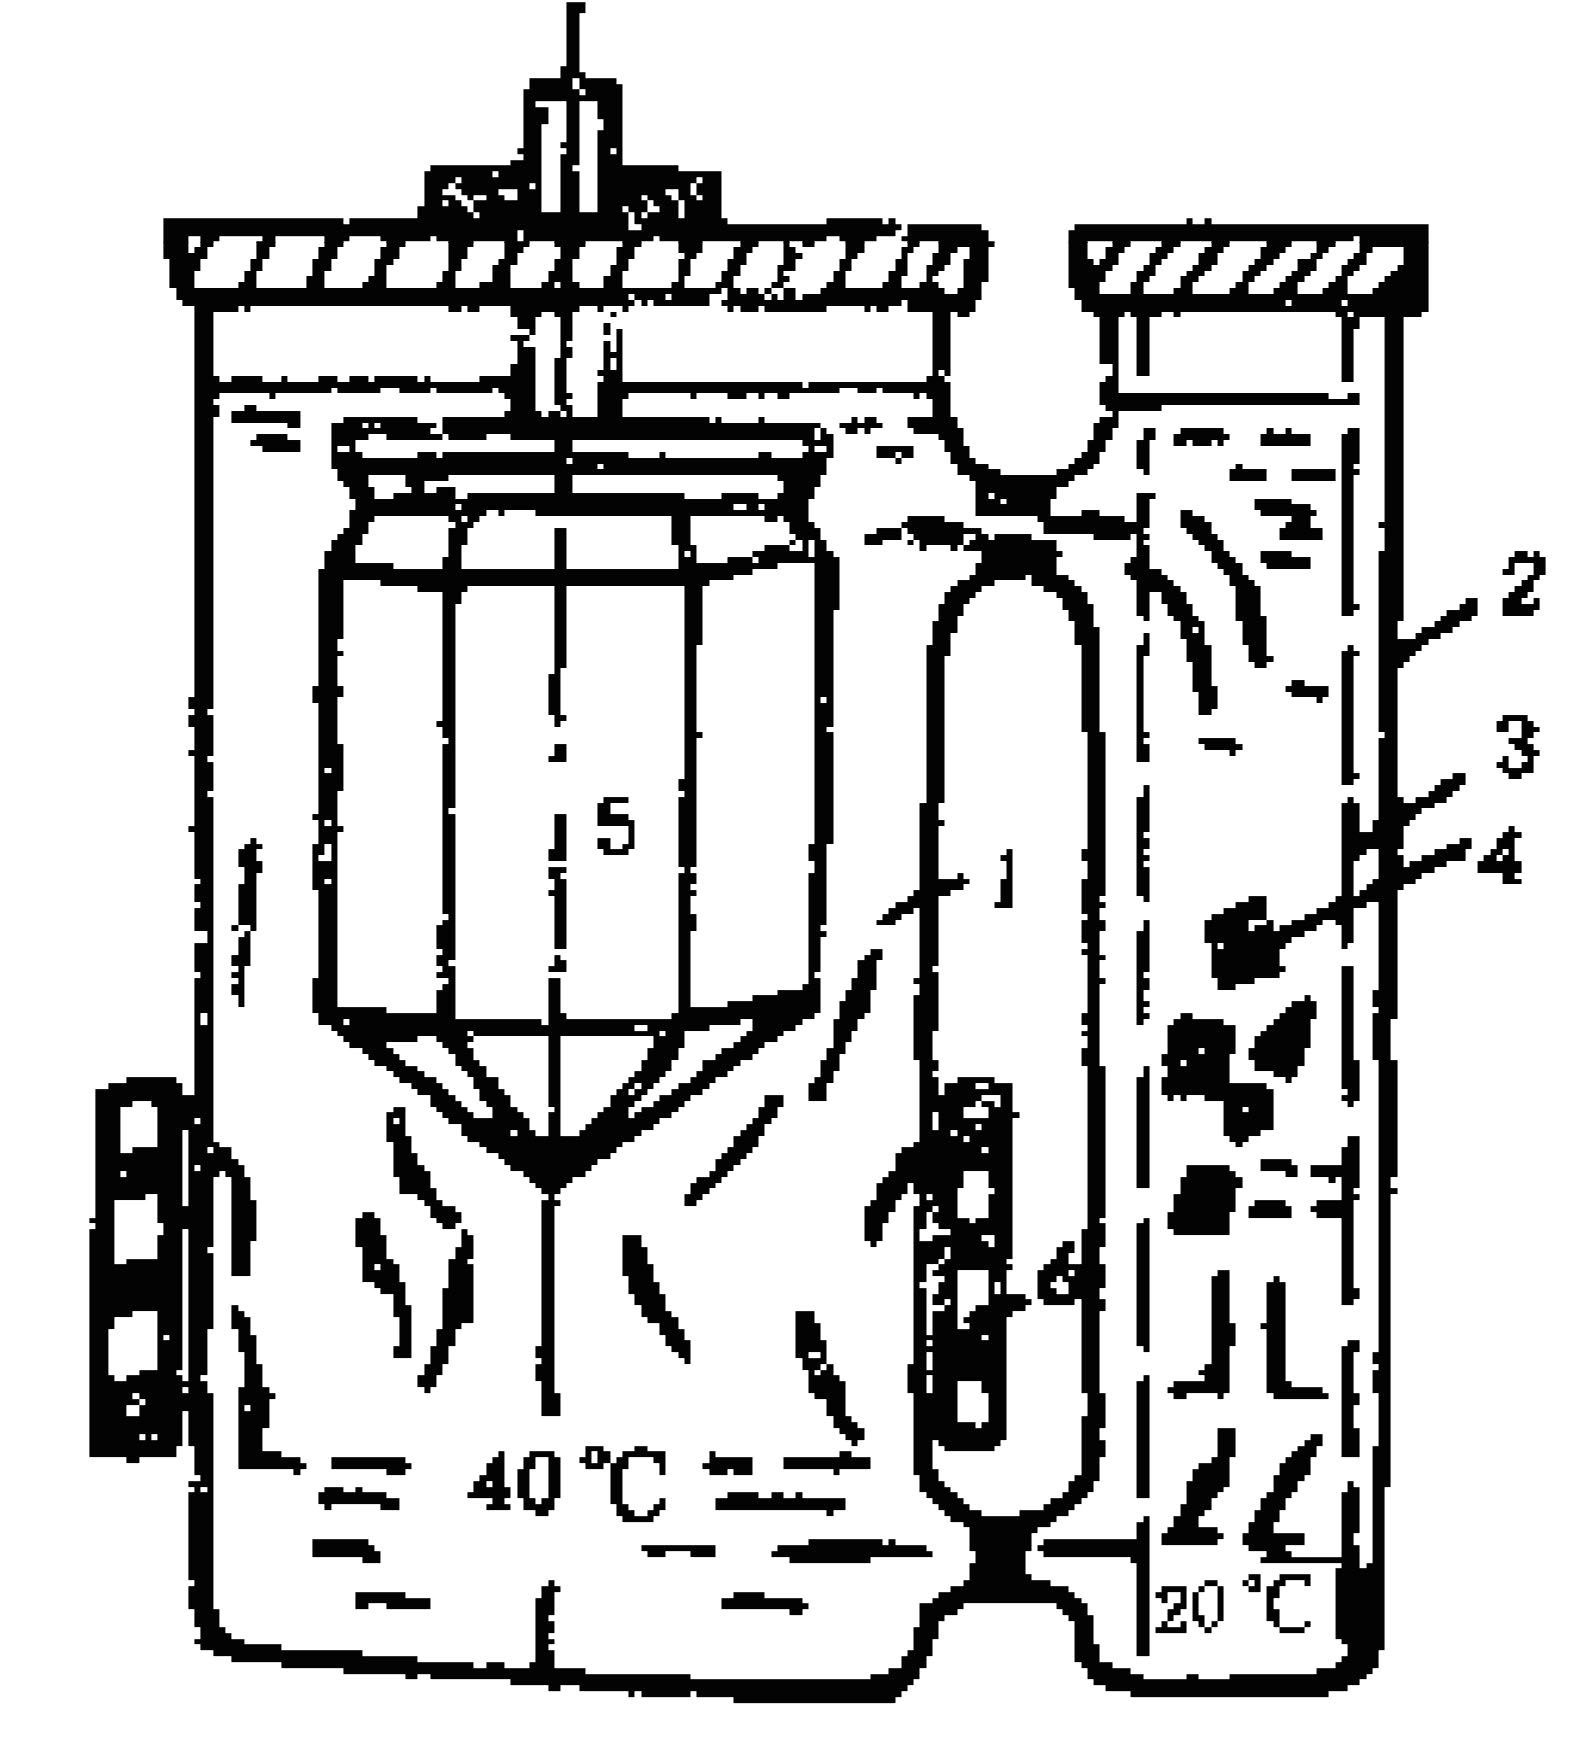
\includegraphics[width=0.5\textwidth]{fig/cp03/img3.22.jpg}
 \caption{浓差对流法生长LiIO$_3$晶体的装置}
\end{figure}